%====================================================
%	CHAPTER 6 - Control & Simulations
%====================================================
\chapter{Simulations and Results}
\label{ch:simulation}
%====================================================
\section{Simulator description}
\label{sec:simulation.block}
%====================================================
The proposed attitude and position control laws, together with the system dynamic equations of motion including each actuator's transfer function, were all tested in simulation to determine a particular controller's efficacy. The rigid-body equations of motion from Sec:\ref{subsec:dynamics.rigidbody.lagrange}, with non-linearities from Sec:\ref{sec:dynamics.aero} and multi-body responses from Sec:\ref{sec:dynamics.nonlinearities}, were incorporated into a high fidelity simulation environment. Closely matching the dynamics of the physical quadrotor prototype proposed in Sec:\ref{sec:proto.design}; relying on measurement data produced by tests in Sec:\ref{subsec:dynamics.nonlinearities.torque-tests} to provide a degree of confidence in the simulations accuracy. The consolidated quaternion dynamics in Sec:\ref{sec:dynamics.model} formed the basis of the simulation; building a loop extended from the control structure in Fig:\ref{fig:control-block}. Each control law is optimized first without the effect of the servo's $180$\textdegree saturation limit. Limiting the servos was a conscientious design decision and as such its effects are investigated in Sec:\ref{sec:simulation.saturation}; but for now servos are considered to be continuous\ldots
\par
\begin{figure}[htbp]
\vspace{-12pt}
\centering
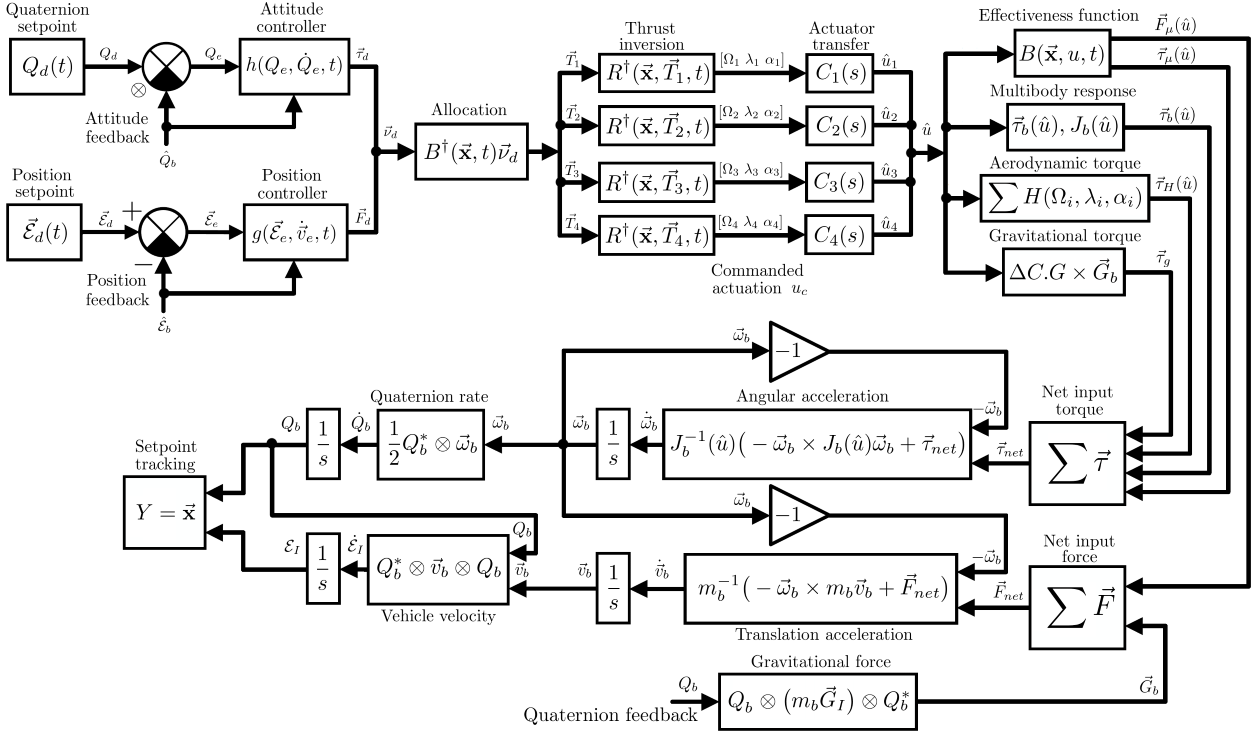
\includegraphics[width=0.93\textwidth]{figs/simulation-block}
\caption{Simulation loop}
\label{fig:simulation-block}
\end{figure}
\vspace{-20pt}
\par
An abstracted simulation block is illustrated in Fig:\ref{fig:simulation-block}; incorporating both attitude and position control loops together with additive non-linearities derived previously. Certain feedback elements were omitted to retain clarity in the diagram, both Coriolis and Gyroscopic non-linear couplings were included. Not shown is some form of state estimation discretization between the state-tracking output $y=\vec{\mathbf{x}}=[Q_b,~\vec{\mathcal{E}}\hspace{2pt}]^T$ and the feedback state $\hat{x}$ used for setpoint tracking. Those effects are discussed subsequently in Sec:\ref{sec:simulation.state}.
\par
Initial conditions for each state integrator, both position and attitude accelerations, $\dot{\vec{v}}_b$ and $\dot{\vec{\omega}}_b$ and their velocities $\dot{\mathcal{E}}$ and $\dot{Q}_b$ respectively, are not illustrated but implied. Obviously starting conditions are important for each trajectory simulation but are explicitly defined for each simulation in question. Actuator transfer functions from Sec:\ref{subsec:proto.design.transfer} are bundled into an $H_{i}(S)$ block to account for the transfer function and saturation effects of each motor module. Each bundled input $u_{1\rightarrow 4}$ is similarly the projected actuator matrix:
\begin{equation}
u_{i}=u\cdot i = \begin{bmatrix}
\Omega_i & \lambda_i & \alpha_i
\end{bmatrix}
\end{equation}
Then $\vec{T}_i(S)$ is the resultant thrust vector from a single motor module with a combined MIMO transfer function. Lastly the setpoints for both attitude and position states are either stepped set points or produced from a simple orbital trajectory. The former is used for controller optimization, discussed subsequently, and the latter is used to evaluate the effective net controller performance. To investigate the question of non-zero setpoint tracking an orbital trajectory is simulated, shown in Fig:\ref{fig:trajectory}
\begin{figure}[htbp]
\centering
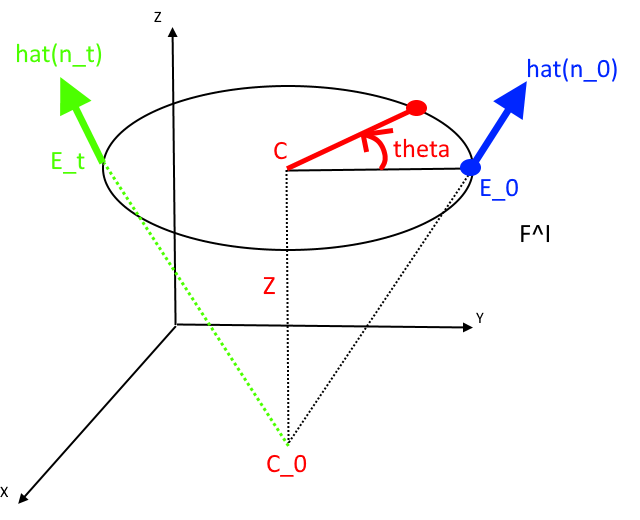
\includegraphics[width=0.5\textwidth]{figs/trajectory}
\caption{Orbital trajectory}
\label{fig:trajectory}
\vspace{-18pt}
\end{figure}
\par
The trajectory's setpoints are exclusively attitude and position targets; the trajectory is independent of actuator values or the aircraft's configuration. For some central point in the inertial frame $\vec{C}_0\in\mathcal{F}^I$, the trajectory orbits at an angular rate of $\dot{\theta}~[\text{Hz}]$ with a height of $\hat{z}_c~[\text{m}]$ at a radius $R~[\text{m}]$ from the center $\vec{C}$. The position setpoint then follows:
\begin{subequations}
\begin{equation}
\vec{\mathcal{E}}_{d}(t)=\begin{bmatrix}
C_{0x}+R\cos \theta(t)\\
C_{0y}+R\sin \theta(t)\\
\hat{z}_c
\end{bmatrix}~~~~\in\mathcal{F}^I
\end{equation}
Every time varying attitude setpoint is aligned with the normal vector $\hat{n}_d(t)$, pointing away from $\vec{C}_0$:
\begin{equation}
\hat{n}_d(t)\triangleq\frac{\vec{\mathcal{E}}_d(t)-\vec{C}_0}{\sqrt{\hat{z}_c^2+R^2}}
\end{equation}
The quaternion setpoint is then constructed such that:
\begin{equation}
Q_d(t)=\begin{bmatrix}
\sin \frac{\theta(t)}{2} & \cos \frac{\theta(t)}{2}\hat{n}_d(t)
\end{bmatrix}^T
\end{equation}
\end{subequations}
No first order or higher derivative setpoints are applied for the trajectory in Fig:\ref{fig:trajectory}. Both position and attitude rates are respectively $\dot{\vec{\mathcal{E}}}_d(t)=\vec{0}$ and $\dot{Q}_d(t)=\vec{0}$ throughout the trajectory.
%====================================================
\section{Controller Tuning}
\label{sec:simulation.tuning}
%====================================================
Control derivation and stability shown previously in Ch:\ref{ch:control} demonstrated only a controller's setpoint tracking ability, providing no further insight into the controller coefficient design. Lyapunov stability theorem, in the context of Sec:\ref{sec:control.attitude}-\ref{sec:control.position}, evaluates a particular trajectory's stability over $t\rightarrow\infty$ but nothing more. Often at the coefficient selection stage a \emph{monte carlo} approach is used; in most cases choosing coefficients seemingly at random and haphazardly, without any obvious forethought\ldots 
%====================================================
\subsection{Partical Swarm Based Optimization}
\label{subsec:simulation.tuning.pso}
%====================================================
Particle swarm based optimization (\emph{PSO}) has been shown in both \cite{adaptivepso} and \cite{autopilotPSO}, amongst others, to be an effective controller coefficient selection tool. The algorithm regards each variable to be optimized as a \emph{particle} which exists within some defined search space. The collection or \emph{swarm} of particles explores the search space directed by both the swarm's previous performance as well as the relative performance between each particle. In \cite{particletrajectories} the statistical nature of the swarm's trajectory is discussed, however such investigations are well beyond the scope of this work.
\par
In general the PSO algorithm applies a directed and \emph{gradient free} based search of solutions for a given optimization problem. The lack of an explicit gradient is an important distinction which differentiates PSO from other algorithms. Often a predefined gradient function is required to direct the optimization search; MatLab's own Fmincon\cite{fmincon} or Interior-Point optimizer\cite{ipopt} algorithms for example. Interval gradient calculations can be computationally exhaustive and reduce the rate of execution for the entire process. An optimizer's performance is directly proportional to the number of iterations it actually executes, if an iteration has a high degree of complexity it's solution time is then adversely effected.
\par
The PSO algorithm is defined as follows; if there exists a set $\vec{x}$ of $k$ variables, $\vec{x}\in\mathbb{R}^{k\times 1}$ to be optimized. The swarm of $\vec{x}_n$ particles at the $n^{\text{th}}$ interval is updated as per the velocity function:
\begin{subequations}
\begin{equation}
\vec{x}_{n+1}=\vec{v}_{n}+x_{n}
\end{equation}
\vspace{-12pt}
\begin{equation}\label{eq:swarm-velocity}
\vec{v}_{n+1}\triangleq w\ast \vec{v}_n+c_1\ast r_1\big(\vec{P}_{best}-\vec{x}_n\big)+c_2\ast r_2\big(\vec{G}_{best}-\vec{x}_n\big)
\end{equation}
\end{subequations}
Each $\ast$ operator in Eq:\ref{eq:swarm-velocity} represents an element-by-element matrix coefficient multiplication operation. Both $\vec{P}_{best}$ and $\vec{G}_{best}$ are previous swarm positions where local and global optima were respectively achieved. Performance of the swarm's current interval is evaluated as per some cost function, responding to a system's dynamics; expanded on next. Finally $r_1$ and $r_2$ are random seeded $\mathbb{R}^{1\times k}$ exploratory matrices which progress the search direction, biased by two weighting coefficients $c_1$ and $c_2$. The search is prejudiced toward local optima by $c_1$ whilst $c_2$ directs the swarm toward global optima. Fig:\ref{fig:swarm-trajectory} illustrates how positions of both local and global optima influence subsequent velocity.
\begin{figure}[hbtp]
\vspace{-12pt}
\centering
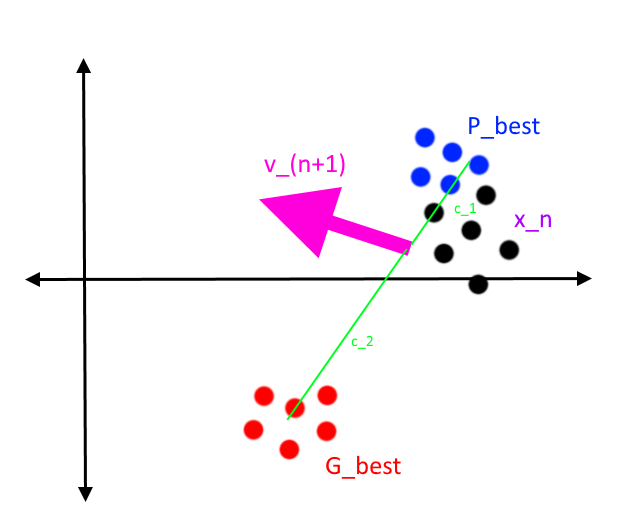
\includegraphics[width=0.47\textwidth]{figs/swarm-trajectory}
\vspace{-12pt}
\caption{Swarm trajectory's velocity direction}
\label{fig:swarm-trajectory}
\end{figure}
\par
The swarm's performance is evaluated by the response of a dynamic system to a particular swarm's interval position; typically an error deviation away from some desired state. Here, the simulation described in Fig:\ref{fig:simulation-block}, is parsed a swarm of controller coefficients as an argument and the plant's response is simulated over a series of setpoint step tests. Particulars with regards to attitude controller optimization is expanded on in Sec:\ref{sec:simulation.attitude} thereafter position controller optimization is detailed in Sec:\ref{sec:simulation.position}. The object is for setpoint tracking so each swarm's coefficient performance metric calculates an integral-time-absolute-error (\emph{ITAE}) cost, \cite{ITAE}.
\begin{equation}
\vec{\zeta}\triangleq\int_{t_0}^{t_\infty}t|\vec{e}(t)|.dt
\end{equation}
With an error $\vec{e}(t)$ deviating from the plant's given setpoint. The ITAE integral is taken over the entire simulation time, an effective $t_\infty$. The time multiplier ensures setpoint error \emph{and} settling time optimality; punishing overshoot and under-damped oscillatory like behaviour.
\par
In general a PSO algorithm follows the flow diagram in Fig:\ref{fig:particle-diagram}. Because each controller was empirically proven to be stable independent of it's trajectory; the controller will settle irrespective of the proposed interval coefficient values. A consequence of this is the starting conditions for the swarm, $\vec{x}_0$, have no bearing on the progression of the optimization. A round set of unity coefficients were selected as a starting point for each controller's optimization\ldots
\begin{figure}[htbp]
\centering
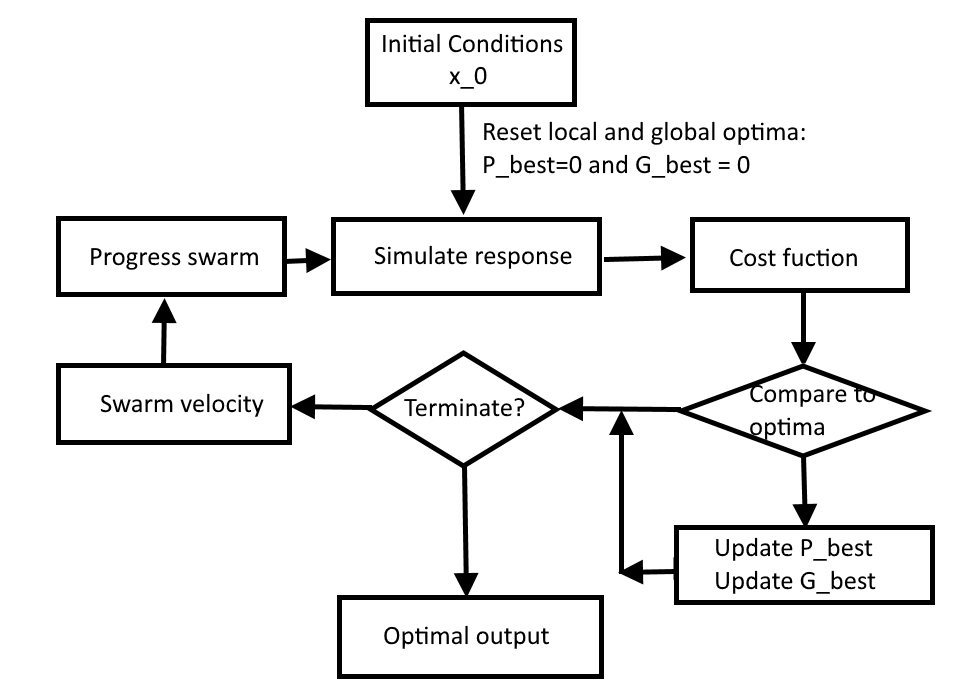
\includegraphics[width=0.7\textwidth]{figs/particle-diagram}
\caption{Particle swarm flow diagram}
\label{fig:particle-diagram}
\end{figure}
\par
Termination conditions for the iterative optimization loop either limit the number of iteration cycles performed or break from the process once a result is regarded as sufficiently close to optimal. Each optimization cycle was iterated for $tx=1000$ times, testing and evaluating one thousand different swarm values for a series of stepped setpoints. As the optimizer progressed through iterations it adapted it's bias from a global to local optima, refining the way in which it searched for potential controller coefficients.
\begin{equation}
\vec{v}_{n+1}=\vec{v}_n+\frac{tx}{1000}\ast r_1(\vec{P}_{best}-\vec{x}_n)+\frac{1000-tx}{1000}\ast r_2(\vec{G}_{best}-\vec{x}_n)
\end{equation}
This provided each controller an equal opportunity to reach optimality and biased control structures which improved their performance at a faster rate. Moreover each swarm's progression was limited such that it never violated the Lyapunov stability conditions of it's pertinent control law\ldots
%====================================================
\section{Attitude Controllers}
\label{sec:simulation.attitude}
%====================================================
Attitude controllers derived in Sec:\ref{sec:control.attitude} were optimized first, owing to their independence from the position loop. A constant hovering force condition was simply applied to the virtual plant input $\vec{F}_d$. A pseudo inversion allocator, Sec:\ref{subsec:allocation.allocators.inverse}, was applied to the control loop when testing each attitude controller. To evaluate an individual swarm's performance a number of step tests were performed. Each attitude setpoint was first defined in the Euler angle parametrization, being conceptually easier to visualize. Thereafter the attitude setpoints were converted into a quaternion attitude and applied to the simulation.
\begin{equation}
\vec{\eta}_d(t)\triangleq \begin{bmatrix}
\phi_d(t)&
\theta_d(t)&
\psi_d(t)
\end{bmatrix}^T\underset{Q}{\iff}Q_d(t)
\end{equation}
Each of the three Euler angles were stepped in the range $[-90\text{\textdegree}:+90\text{\textdegree}]$ at an interval of $30\text{\textdegree}$. This resulted in a test of 343 possible attitude setpoints; making a workspace sphere as shown in Fig:\ref{fig:attitude-setpoint}. The attitude steps were given $t=15~[\text{s}]$ to reach their settling point, with an initial attitude position always at the origin $Q_b(t_0)=[1~\vec{0}\hspace{2pt}]$, with a \emph{positive} quaternion scalar. The performance metric for each attitude step test was an ITAE integral of quaternion vector and angular velocity errors:
\begin{equation}\label{eq:attitude-performance}
\vec{\zeta}_{Q}=C_Q\int_{t=0}^{15}t|\vec{q}_e(t)|.dt+C_\omega\int_{t=0}^{15}t|\vec{\omega}_e(t)|.dt~~~~\in\mathbb{R}^{3}
\end{equation}
Weighting coefficients $C_Q$ and $Q_\omega$ balance priority of either quaternion or angular velocity tracking, however, tracking both were equally important and so those weights were $C_Q=Q_\omega=1$. The cost integral in Eq:\ref{eq:attitude-performance} was averaged over all 343 possible attitude steps to ascertain the overall performance of a proposed set of coefficients.
\begin{figure}[htbp]
\centering
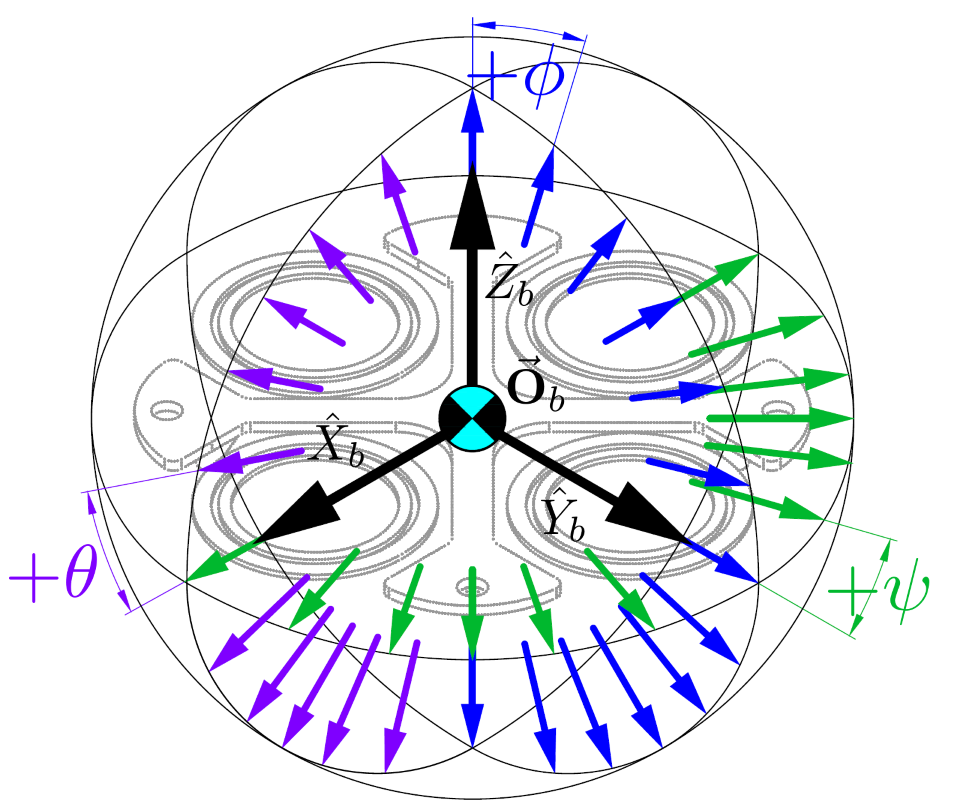
\includegraphics[width=0.7\textwidth]{figs/attitude-setpoint}
\caption{Attitude setpoint working space}
\label{fig:attitude-setpoint}
\end{figure}
\par
The integral in Eq:\ref{eq:attitude-performance} produces a vector $\in\mathbb{R}^{3}$ result. Each coefficient in a particular controller contributes towards a local error in one of the $\hat{X},\hat{Y},\hat{Z}$ components, or in certain cases a pair of axial components. Each controller's local errors and the coefficients which affect them are discussed subsequently. A global error for the performance of each controller is simply the magnitude of $\norm{\vec{\zeta}_Q}$. That same global error is applicable to all of the controllers\ldots
\newpage
To compare the relative performance and effectiveness of each optimized control structure a single attitude step was investigated. That attitude change was chosen to be a sizeable step in all three Euler angles:
\begin{equation}\label{eq:attitude-step-position}
\vec{\eta}_d=\begin{bmatrix}
\phi_d\\
\theta_d\\
\psi_d\\
\end{bmatrix}
=
\begin{bmatrix*}[r]
-142\text{\textdegree}\\
167\text{\textdegree}\\
-45\text{\textdegree}
\end{bmatrix*}
\underset{Q}{\iff}
\begin{bmatrix}
-0.3254&
0.2226&
-0.2579&
0.8821
\end{bmatrix}^T
\end{equation}
Then each controller's settling time, $t_{95}$, and it's relative angular velocity (the setpoint for which is $\vec{|omega}_d=\vec{0}$) for such a step is evaluated. Settling time, overshoot and setpoint error are all factors to consider when discussing the performance of a control law. Lastly, the commanded virtual input torque to the actuator set is considered too, a feasible controller can not command torque saturation or unachievable input rate changes.
%====================================================
\subsection{PD}
\label{subsec:simulation.attitude.pd}
%====================================================
The first controller evaluated, the Proportional-Derivative structure, investigates three different scenarios. Before discussing those different situations, it is worth recalling that control structure from Sec:\ref{subsubsec:control.attitude.controllers.pd}. The control torque is designed:
\begin{equation}\label{eq:simulation-attitde-pd}
\vec{\tau}_{_{PD}}=\underbrace{K_p\vec{q}_e+K_d\vec{\omega}_e}_{Independent}+\underbrace{\vec{\omega}_b\times J_b(u)\vec{\omega}_b+\hat{\tau}_b(u)-\vec{\tau}_g-\vec{\tau}_Q}_{Compensation}~~~~\in\mathcal{F}^{b}
\end{equation}
The first two cases regard both coefficient matrices as purely diagonal, with no skew elements; testing the effect of plant dependent compensation on the controller's performance. Lastly a plant dependent compensating PD controller is tested \emph{with} symmetrical coefficient matrices. When the coefficient matrices are both diagonal the case follows:
\begin{equation}\label{eq:simulation-attitde-pd-diagonal-coefficients}
K_p\triangleq \begin{bmatrix}
K_p(1) & 0 & 0\\
0 & K_p(2) & 0\\
0 & 0 & K_p(3)
\end{bmatrix}
~~\text{and}~~K_d\triangleq \begin{bmatrix}
K_d(1) & 0 & 0\\
0 & K_d(2) & 0\\
0 & 0 & K_d(3)
\end{bmatrix}
\end{equation}
The local and global coefficient best positions are found respectively such that:
\begin{equation}
\vec{P}_{Best}\equiv
\begin{bmatrix}
K_p(1)\Rightarrow \min \vec{q}_e(1)\\
K_p(2)\Rightarrow \min \vec{q}_e(2)\\
K_p(3)\Rightarrow \min \vec{q}_e(3)\\
K_d(1)\Rightarrow \min \vec{\omega}_e(1)\\
K_d(2)\Rightarrow \min \vec{\omega}_e(2)\\
K_d(3)\Rightarrow \min \vec{\omega}_e(3)
\end{bmatrix}~~\text{and}~~\vec{G}_{Best}\equiv\begin{bmatrix}
K_p(1)\Rightarrow \min \vec{\zeta}_{_{PD}}(1)\\
K_p(2)\Rightarrow \min \vec{\zeta}_{_{PD}}(2)\\
K_p(3)\Rightarrow \min \vec{\zeta}_{_{PD}}(3)\\
K_d(1)\Rightarrow \min \vec{\zeta}_{_{PD}}(1)\\
K_d(2)\Rightarrow \min \vec{\zeta}_{_{PD}}(2)\\
K_d(3)\Rightarrow \min \vec{\zeta}_{_{PD}}(3)
\end{bmatrix}
\end{equation}
In the symmetrical coefficient case, the controller coefficients are then numbered:
\begin{equation}\label{eq:simulation-attitde-pd-symmetric-coefficients}
K_p\triangleq \begin{bmatrix}
K_p(1) & K_p(4) & K_p(5)\\
K_p(4) & K_p(2) & K_p(6)\\
K_p(5) & K_p(6) & K_p(3)
\end{bmatrix}
~~\text{and}~~K_d\triangleq \begin{bmatrix}
K_d(1) & K_d(4) & K_d(5)\\
K_d(4) & K_d(2) & K_d(6)\\
K_d(5) & K_d(6) & K_d(3)
\end{bmatrix}
\end{equation}
Where it's local and global coefficient positions are then found such that:
\begin{subequations}\label{eq:simulation-attitude-pd-symmetric-best}
\begin{equation}
\vec{P}_{Best}\equiv
\begin{bmatrix}
K_p(1)\Rightarrow \min \vec{q}_e(1) & K_p(4)\Rightarrow \min \vec{q}_e(1)\&\&\vec{q}_e(2)\\
K_p(2)\Rightarrow \min \vec{q}_e(2)& K_p(5)\Rightarrow \min\vec{q}_e(1)\&\&\vec{q}_e(3) \\
K_p(3)\Rightarrow \min \vec{q}_e(3) & K_p(6)\Rightarrow \min\vec{q}_e(2)\&\&\vec{q}_e(3)\\
K_d(1)\Rightarrow \min \vec{\omega}_e(1) & K_d(4)\Rightarrow \min\vec{\omega}_e(1)\&\&\vec{\omega}_e(2)\\
K_d(2)\Rightarrow \min \vec{\omega}_e(2) & K_d(5)\Rightarrow\min\vec{\omega}_e(1)\&\&\vec{\omega}_e(3)\\
K_d(3)\Rightarrow \min \vec{\omega}_e(3)& K_d(6)\Rightarrow\min\vec{\omega}_e(2)\&\&\vec{\omega}_e(3)
\end{bmatrix}
\end{equation}
\begin{equation}
\vec{G}_{Best}\equiv\begin{bmatrix}
K_p(1)\Rightarrow \min \vec{\zeta}_{_{PD}}(1) & K_p(4)\Rightarrow\min\vec{\zeta}_{_{PD}}(1)\&\& \vec{\zeta}_{_{PD}}(2)\\
K_p(2)\Rightarrow \min \vec{\zeta}_{_{PD}}(2) & K_p(5)\Rightarrow\min\vec{\zeta}_{_{PD}}(1)\&\& \vec{\zeta}_{_{PD}}(3)\\
K_p(3)\Rightarrow \min \vec{\zeta}_{_{PD}}(3) & K_p(6)\Rightarrow\min\vec{\zeta}_{_{PD}}(2)\&\& \vec{\zeta}_{_{PD}}(3)\\
K_d(1)\Rightarrow \min \vec{\zeta}_{_{PD}}(1) & K_d(4)\Rightarrow\min\vec{\zeta}_{_{PD}}(1)\&\& \vec{\zeta}_{_{PD}}(2)\\
K_d(2)\Rightarrow \min \vec{\zeta}_{_{PD}}(2) & K_d(5)\Rightarrow\min\vec{\zeta}_{_{PD}}(1)\&\& \vec{\zeta}_{_{PD}}(3)\\
K_d(3)\Rightarrow \min \vec{\zeta}_{_{PD}}(3) & K_d(6)\Rightarrow\min\vec{\zeta}_{_{PD}}(2)\&\& \vec{\zeta}_{_{PD}}(3)\\
\end{bmatrix}
\end{equation}
\end{subequations}
%====================================================
\subsubsection{Independent Performance}
\label{subsubsec:simulation.atttiude.pd.independent}
%====================================================
For the independent case, the same coefficients are used as those for the plant dependent case. The compensation terms in Eq:\ref{eq:simulation-attitde-pd} are neglected to produce a plant independent controller. Optimizing the diagonal only PD controller produced the following coefficients:
\begin{equation}\label{eq:optimized-pd-independent}
K_p = \begin{bmatrix}
3.5679 & 0 & 0\\
0 & 5.2698 & 0\\
0 & 0 & 6.0695
\end{bmatrix}
~~\text{and}~~K_d = \begin{bmatrix}
9.0150 & 0 & 0\\
0 & 11.4848 & 0\\
0 & 0 & 20.1827
\end{bmatrix}
\end{equation}
Fig:\ref{fig:PD_Diagonal_Independent_Step} plots the quaternion response to an attitude step described in Eq:\ref{eq:attitude-step-position}. The uncompensated plant never actually settles to the setpoint; a constant steady state error manifests as a result of the uncompensated dynamics. The plant does, however, stablize at $t = 3.35~[\text{s}]$. Fig:\ref{fig:PD_Diagonal_Independent_Torque} shows the designed and commanded torques $\vec{\tau}_d$ and $\vec{\tau}_c$ respectively. The actuator transfer functions produce a lagging response on those inputs. Lastly Fig:\ref{fig:PD_Diagonal_Independent_Angular} shows the body's angular velocity $\vec{\omega}_b$ which steps to apply an attitude rotation. 
\begin{figure}[htbp]
\centering
\begin{subfigure}{\textwidth}
\centering
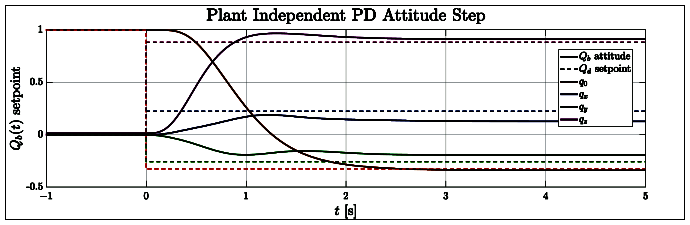
\includegraphics[width=0.65\textwidth]{graphs/PD_Diagonal_Independent_Step}
\caption{Quaternion attitude step}
\label{fig:PD_Diagonal_Independent_Step}
\end{subfigure}
\begin{subfigure}{0.49\textwidth}
\centering
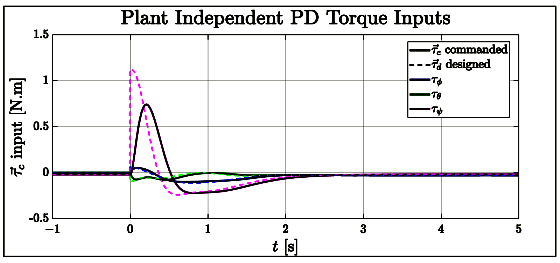
\includegraphics[width=\textwidth]{graphs/PD_Diagonal_Independent_Torque}
\caption{Plant input torques}
\label{fig:PD_Diagonal_Independent_Torque}
\end{subfigure}
\begin{subfigure}{0.49\textwidth}
\centering
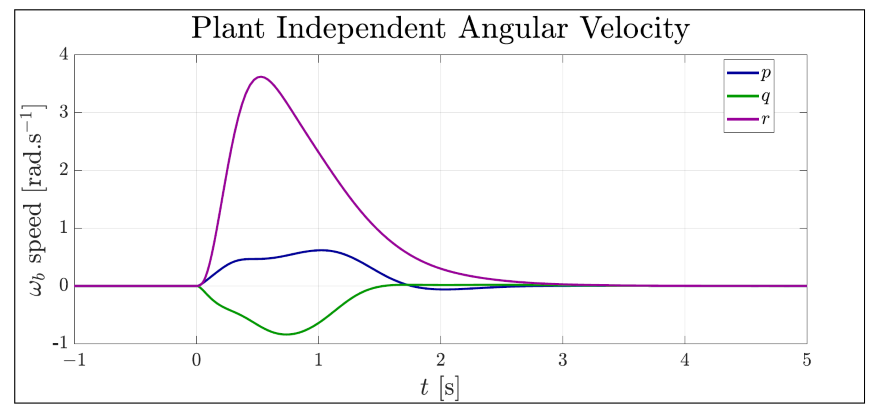
\includegraphics[width=\textwidth]{graphs/PD_Diagonal_Independent_Angular}
\caption{Angular velocity}
\label{fig:PD_Diagonal_Independent_Angular}
\end{subfigure}
\caption{Independent diagonal PD}
\end{figure}
%====================================================
\subsubsection{Dependent Performance}
\label{subsubsec:simulation.atttiude.pd.dependent}
%====================================================
The inclusion of a plant independent PD controller is purely for the sake of contrition, showing that a plant dependency is needed to account for steady state tracking errors. The same controller coefficients from Eq:\ref{eq:optimized-pd-independent} are used now to test the controller's dependent case; wherein the controller compensates for plant dynamics with a feedback terms.
\par
Fig:\ref{fig:PD_Diagonal_Dependent_Step} shows the quaternion attitude step for the plant dependent case. The attitude settles in $t_{95}=3.0764~[\text{s}]$. The dynamic response is much the same as the independent one previously in Fig:\ref{fig:PD_Diagonal_Independent_Step}. The torque input is still within the feasible range, not saturating any actuators. The difference is that at steady state the plant's torque input is slightly non-zero, to compensate for the previous steady state error.
\par
\begin{figure}[htbp]
\centering
\begin{subfigure}{\textwidth}
\centering
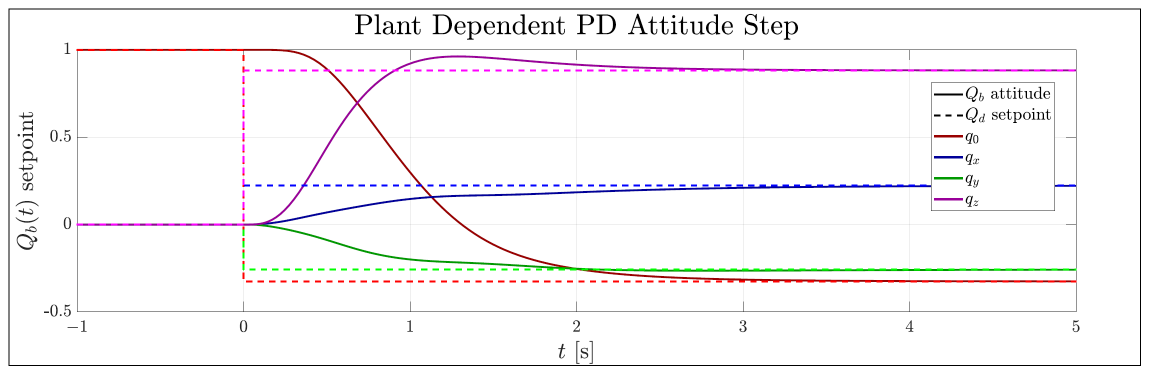
\includegraphics[width=0.65\textwidth]{graphs/PD_Diagonal_Dependent_Step}
\caption{Quaternion attitude step}
\label{fig:PD_Diagonal_Dependent_Step}
\end{subfigure}
\begin{subfigure}{0.49\textwidth}
\centering
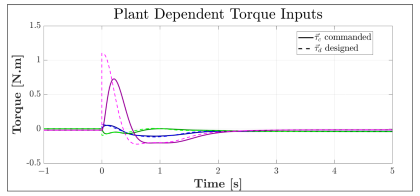
\includegraphics[width=\textwidth]{graphs/PD_Diagonal_Dependent_Torque}
\caption{Plant input torques}
\label{fig:PD_Diagonal_Dependent_Torque}
\end{subfigure}
\begin{subfigure}{0.49\textwidth}
\centering
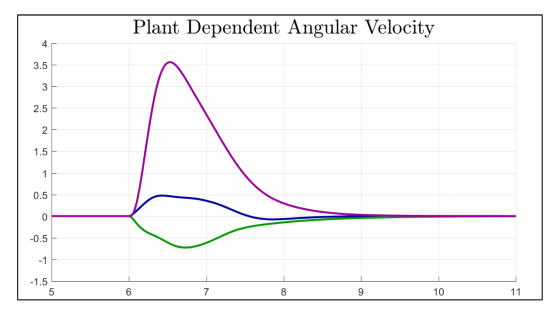
\includegraphics[width=\textwidth]{graphs/PD_Diagonal_Dependent_Angular}
\caption{Angular velocity}
\label{fig:PD_Diagonal_Dependent_Angular}
\end{subfigure}
\caption{Dependent diagonal PD}
\end{figure}
%====================================================
\subsubsection{Symmetric Controller Performance}
\label{subsubsec:simulation.atttiude.pd.3x3}
%====================================================
The final Proportional-Derivative attitude controller considers both coefficient matrices with non-zero off-diagonal skew elements. Eq:\ref{eq:simulation-attitde-pd-symmetric-coefficients} shows the structure for both matrices. Once optimized the controller coefficients numeric values are:
\begin{equation}\label{eq:optimized-pd-symmetric}
K_p = \begin{bmatrix}
5.9157 & 0.41649 & 0.47138\\
0.41649 & 7.3141 & 0.49448\\
0.47138 & 0.49448 & 7.3135
\end{bmatrix}
~~\text{and}~~K_d = \begin{bmatrix}
17.4318 & 0.453106 & 0.152577\\
0.453106 & 15.3569 & 0.577193\\
0.152577 & 0.577193 & 26.3436
\end{bmatrix}
\end{equation}
The first difference presented with the symmetric controller coefficients is that the effective gain applied by Eq:\ref{eq:optimized-pd-symmetric} is significantly greater than that of Eq:\ref{eq:optimized-pd-independent}. The off-diagonal elements are tending towards "undoing" the cross coupling as a result of the Gyroscopic torque induced in Eq:\ref{eq:quaternion-states-angular}. 
\par
Fig:\ref{fig:PD_3x3_Dependent_Step} shows the step response of the symmetric PD controller. The increased effective gain in Eq:\ref{eq:optimized-pd-symmetric} results in larger overshoot and an increased settling time, $t_{95}=3.2993~[\text{s}]$. Neither greater commanded torque, Fig:\ref{fig:PD_3x3_Dependent_Torque}, nor an increased angular velocity spike, Fig:\ref{fig:PD_3x3_Dependent_Angular} are altogether unexpected consequences of a more aggressive control law. The increased number of coefficients to be tuned imply that the optimization applied to produce Eq:\ref{eq:optimized-pd-symmetric} was perhaps not as effective as reducing step errors as that of the diagonal Eq:\ref{eq:optimized-pd-independent}.
\begin{figure}[htbp]
\centering
\begin{subfigure}{\textwidth}
\centering
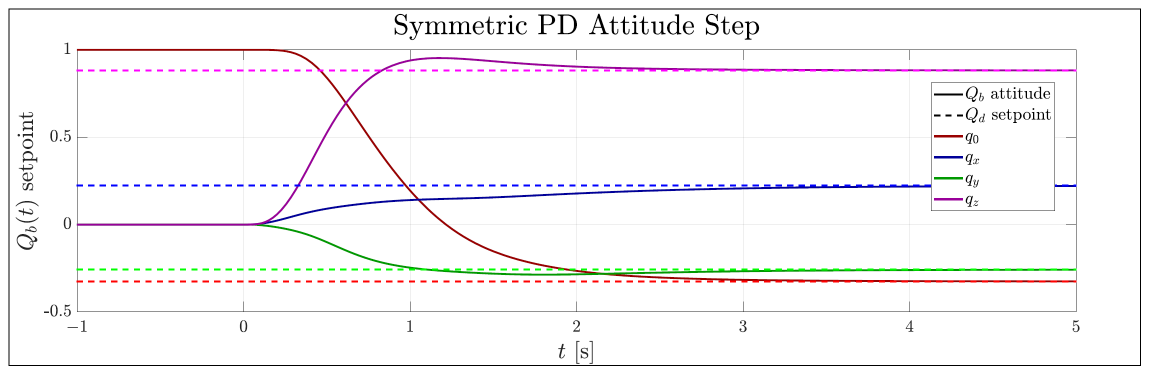
\includegraphics[width=0.65\textwidth]{graphs/PD_3x3_Dependent_Step}
\caption{Quaternion attitude step}
\label{fig:PD_3x3_Dependent_Step}
\end{subfigure}
\begin{subfigure}{0.49\textwidth}
\centering
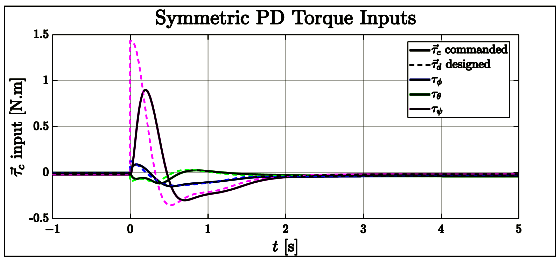
\includegraphics[width=\textwidth]{graphs/PD_3x3_Dependent_Torque}
\caption{Plant input torques}
\label{fig:PD_3x3_Dependent_Torque}
\end{subfigure}
\begin{subfigure}{0.49\textwidth}
\centering
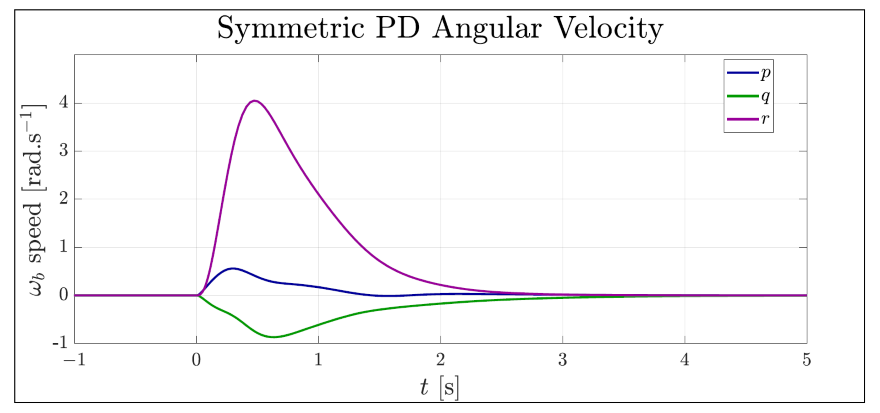
\includegraphics[width=\textwidth]{graphs/PD_3x3_Dependent_Angular}
\caption{Angular velocity}
\label{fig:PD_3x3_Dependent_Angular}
\end{subfigure}
\caption{Dependent symmetric PD}
\end{figure}
%====================================================
\subsection{Auxilliary Plant Controller}
\label{subsec:simulation.attitude.xpd}
%====================================================
The first of two exponentially stable controllers is the Auxilliary Plant controller from Sec:\ref{subsubsec:control.attitude.controllers.auxpd}. Recalling the simplified controller structure from Eq:\ref{eq:control-aux-pd}:
\begin{equation}\label{eq:simulation-attitude-auxpd}
\vec{\tau}_{_{XPD}}=\underbrace{\Gamma_2{\widetilde{\Omega}}+\Gamma_3\vec{q}_e-J_b(u)\dot{\bar{\Omega}}}_{Independent}+\underbrace{\vec{\omega}_b\times J_b(u)\vec{\omega}_b+\hat{\tau}_b(u)-\vec{\tau}_g-\vec{\tau}_Q}_{Compensation}
\end{equation}
In Eq:\ref{eq:simulation-attitude-auxpd} both coefficient matrix's $\Gamma_2$ and $\Gamma_3$ and diagonal, whereas $\Gamma_1$ is a symmetrical $3\times 3$ gain matrix. Those coefficients are then structured as follows:
\begin{multline}\label{eq:simulation-attitde-auxpd-coefficients}
\Gamma_1\triangleq \begin{bmatrix}
\Gamma_1(1) & \Gamma_1(4) & \Gamma_1(5)\\
\Gamma_1(4) & \Gamma_1(2) & \Gamma_1(6)\\
\Gamma_1(5) & \Gamma_1(6) & \Gamma_1(3)
\end{bmatrix}~,~~
\Gamma_2\triangleq \begin{bmatrix}
\Gamma_2(1) & 0 & 0\\
0 &\Gamma_2(2) & 0\\
0 & 0 & \Gamma_2(3)
\end{bmatrix}
\\
~~\text{and}~~\Gamma_3\triangleq \begin{bmatrix}
\Gamma_3(1) & 0 & 0\\
0 & \Gamma_3(2) & 0\\
0 & 0 & \Gamma_3(3)
\end{bmatrix}
\end{multline}
From the error states on which coefficients in Eq:\ref{eq:simulation-attitde-auxpd-coefficients} act on, the local and globally optimum coefficient positions are found. The first coefficient $\Gamma_1$ acts on both $\vec{q}_e$ and $\vec{\omega}_e$ so it's local errors are also global errors. The remaining coefficient matrices $\Gamma_2$ and $\Gamma_3$ act on $\vec{q}_e$ and $\vec{\omega}_e$ respectively. The local best swarm position is then found:
\begin{subequations}
\begin{equation}
\vec{P}_{Best}\equiv
\begin{bmatrix}
\Gamma_1(1)\Rightarrow \min \vec{\zeta}_{_{XPD}}(1) & \Gamma_1(4)\Rightarrow\min\vec{\zeta}_{_{XPD}}(1)\&\& \vec{\zeta}_{_{XPD}}(2)\\
\Gamma_1(2)\Rightarrow \min \vec{\zeta}_{_{PXD}}(2) & \Gamma_1(5)\Rightarrow\min\vec{\zeta}_{_{XPD}}(1)\&\& \vec{\zeta}_{_{XPD}}(3)\\
\Gamma_1(3)\Rightarrow \min \vec{\zeta}_{_{XPD}}(3) & \Gamma_1(6)\Rightarrow\min\vec{\zeta}_{_{XPD}}(2)\&\& \vec{\zeta}_{_{XPD}}(3)\\
\Gamma_2(1)\Rightarrow \min \vec{q}_e(1) & \Gamma_3(1)\Rightarrow\min\vec{\omega}_e(1)\\
\Gamma_2(2)\Rightarrow \min \vec{q}_e(2) & \Gamma_3(2)\Rightarrow\min\vec{\omega}_e(2)\\
\Gamma_2(3)\Rightarrow \min \vec{q}_e(3) & \Gamma_3(3)\Rightarrow\min\vec{\omega}_e(3)\\
\end{bmatrix}
\end{equation}
The global best swarm position is found similarly:
\begin{equation}
\vec{G}_{Best}\equiv
\begin{bmatrix}
\Gamma_1(1)\Rightarrow \min \vec{\zeta}_{_{XPD}}(1) & \Gamma_1(4)\Rightarrow\min\vec{\zeta}_{_{XPD}}(1)\&\& \vec{\zeta}_{_{XPD}}(2)\\
\Gamma_1(2)\Rightarrow \min \vec{\zeta}_{_{PXD}}(2) & \Gamma_1(5)\Rightarrow\min\vec{\zeta}_{_{XPD}}(1)\&\& \vec{\zeta}_{_{XPD}}(3)\\
\Gamma_1(3)\Rightarrow \min \vec{\zeta}_{_{XPD}}(3) & \Gamma_1(6)\Rightarrow\min\vec{\zeta}_{_{XPD}}(2)\&\& \vec{\zeta}_{_{XPD}}(3)\\
\Gamma_2(1)\Rightarrow \min \vec{\zeta}_{_{XPD}}(1) & \Gamma_3(1)\Rightarrow\min\vec{\zeta}_{_{XPD}}(1)\\
\Gamma_2(2)\Rightarrow \min \vec{\zeta}_{_{XPD}}(2) & \Gamma_3(2)\Rightarrow\min\vec{\zeta}_{_{XPD}}(2)\\
\Gamma_2(3)\Rightarrow \min \vec{\zeta}_{_{XPD}}(3) & \Gamma_3(3)\Rightarrow\min\vec{\zeta}_{_{XPD}}(3)\\
\end{bmatrix}
\end{equation}
\end{subequations} 
The optimized control coefficients, after $tx=1000$ iterations, were as follows:
\begin{multline}\label{eq:optimized-auxpd}
\Gamma_1=\begin{bmatrix}
3.5924 & -0.2457 & -0.027699\\
-0.2457 & 3.0666 & -0.06023\\
-0.027699 & -0.06023 & -3.3809
\end{bmatrix}~,~~\Gamma_2=\begin{bmatrix}
4.6943 & 0 & 0\\
0 & 4.1642 & 0\\
0 & 0 & 6.4109
\end{bmatrix}\\
~~\text{and}~~\Gamma_3=\begin{bmatrix}
1.1007 & 0 & 0\\
0 & 1.3369 & 0 \\
0 & 0 & 1.1331
\end{bmatrix}
\end{multline}
Aside from the added exponential stability, another distinctive feature of the control structure in Eq:\ref{eq:simulation-attitde-auxpd-coefficients} is a significant added complexity. Each optimization iteration took notably longer to complete than the simpler PD controller, in the order of 50-60\% increased simulation times per iteration. Fig:\ref{fig:XPD_Step} shows the quaternion attitude step for the present control structure. It reaches a settling point $t_{95}=2.3688~[\text{s}]$, a significant improvement compared to previous results. That improved attitude step time does come at the cost of greater input torques, shown in Fig:\ref{fig:XPD_Torque}, but still not as costly as a symmetric PD controller. Moreover Fig:\ref{fig:XPD_Angular} shows a greater sustained angular velocity $\vec{\omega}_b$ but with a smoother rate applied to it. 
\par
\begin{figure}[hbtp]
\centering
\begin{subfigure}{\textwidth}
\centering
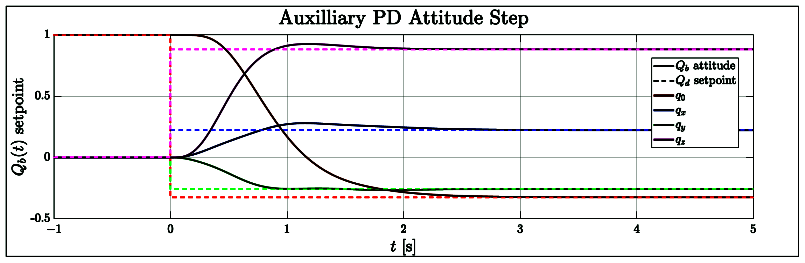
\includegraphics[width=0.65\textwidth]{graphs/XPD_Step}
\caption{Quaternion attitude step}
\label{fig:XPD_Step}
\end{subfigure}
\end{figure}
\par
\begin{figure}[htbp]\ContinuedFloat
\begin{subfigure}{0.49\textwidth}
\centering
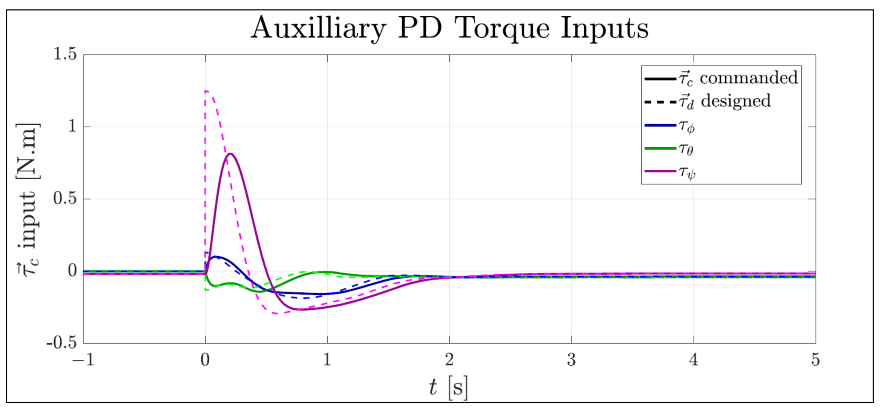
\includegraphics[width=\textwidth]{graphs/XPD_Torque}
\caption{Plant input torques}
\label{fig:XPD_Torque}
\end{subfigure}
\begin{subfigure}{0.49\textwidth}
\centering
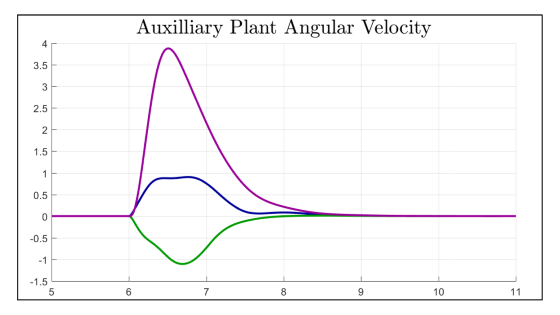
\includegraphics[width=\textwidth]{graphs/XPD_Angular}
\caption{Angular velocity}
\label{fig:XPD_Angular}
\end{subfigure}
\caption{Auxilliary plant controller}
\end{figure}
%====================================================
\subsection{Ideal and Adaptive Backstepping Controllers}
%====================================================
The final attitude control structure to test is that of the Ideal Backstepping Controller. Both Ideal and Adaptive backstepping controllers use the same shared optimized coefficients, the structural difference is that an adaptive disturbance observer applies compensation in the latter control to improve robust stability. Recalling the IBC structure from Eq:\ref{eq:control-ibc};
\begin{equation}\label{eq:simulation-attitude-ibc}
=\underbrace{J_b(u)\Big((\Gamma_1\Gamma_2+1)\vec{q}_e-\Gamma_2\vec{\omega}_b+\Gamma_1\dot{\vec{q}}_e \Big)}_{\text{Ideal backstepping}}
+\underbrace{\vec{\omega}_b\times J_b(u)\vec{\omega}_b+\hat{\tau}_b(u)-\vec{\tau}_g-\vec{\tau}_Q}_{\text{Compenstation}}~~~~\in\mathcal{F}^{b}
\end{equation}
Both gain matrices $\Gamma_1$ and $\Gamma_2$ are positive symmetrical $3\times 3$ coefficient matrices:
\begin{equation}\label{eq:simulation-attitde-ibc-coefficients}
\Gamma_1\triangleq \begin{bmatrix}
\Gamma_1(1) & \Gamma_1(4) & \Gamma_1(5)\\
\Gamma_1(4) & \Gamma_1(2) & \Gamma_1(6)\\
\Gamma_1(5) & \Gamma_1(6) & \Gamma_1(3)
\end{bmatrix}
~~\text{and}~~
\Gamma_2\triangleq \begin{bmatrix}
\Gamma_2(1) & \Gamma_2(4) & \Gamma_2(5)\\
\Gamma_2(4) & \Gamma_2(2) & \Gamma_2(6)\\
\Gamma_2(5) & \Gamma_2(6) & \Gamma_2(3)
\end{bmatrix}
\end{equation}
However, both sets of coefficients act on $\vec{q}_e$ and $\vec{\omega}_e$. As a result the local and global coefficient optimum positions are one in the same. This reduces the directed swarm search to an effective \emph{monte carlo} trial and error scenario. To avoid this it was decided to prioritize $\Gamma_1$ to $\vec{q}_e$ and $\Gamma_2$ to $\vec{\omega}_e$. It then follows that such positions are found in a similar way to the symmetrical PD controller, Eq:\ref{eq:simulation-attitude-pd-symmetric-best}. That means local and global positions can still be used to direct the search space:
\begin{subequations}
\begin{equation}
\vec{P}_{Best}\equiv
\begin{bmatrix}
\Gamma_1(1)\Rightarrow \min \vec{q}_e(1) & \Gamma_1(4)\Rightarrow \min \vec{q}_e(1)\&\&\vec{q}_e(2)\\
\Gamma_1(2)\Rightarrow \min \vec{q}_e(2)& \Gamma_1(5)\Rightarrow \min\vec{q}_e(1)\&\&\vec{q}_e(3) \\
\Gamma_1(3)\Rightarrow \min \vec{q}_e(3) & \Gamma_1(6)\Rightarrow \min\vec{q}_e(2)\&\&\vec{q}_e(3)\\
\Gamma_2(1)\Rightarrow \min \vec{\omega}_e(1) & \Gamma_2(4)\Rightarrow \min\vec{\omega}_e(1)\&\&\vec{\omega}_e(2)\\
\Gamma_2(2)\Rightarrow \min \vec{\omega}_e(2) & \Gamma_2(5)\Rightarrow\min\vec{\omega}_e(1)\&\&\vec{\omega}_e(3)\\
\Gamma_2(3)\Rightarrow \min \vec{\omega}_e(3)& \Gamma_2(6)\Rightarrow\min\vec{\omega}_e(2)\&\&\vec{\omega}_e(3)
\end{bmatrix}
\end{equation}
\begin{equation}
\vec{G}_{Best}\equiv\begin{bmatrix}
\Gamma_1(1)\Rightarrow \min \vec{\zeta}_{_{IBC}}(1) & \Gamma_1(4)\Rightarrow\min\vec{\zeta}_{_{IBC}}(1)\&\& \vec{\zeta}_{_{IBC}}(2)\\
\Gamma_1(2)\Rightarrow \min \vec{\zeta}_{_{IBC}}(2) & \Gamma_1(5)\Rightarrow\min\vec{\zeta}_{_{IBC}}(1)\&\& \vec{\zeta}_{_{IBC}}(3)\\
\Gamma_1(3)\Rightarrow \min \vec{\zeta}_{_{IBC}}(3) & \Gamma_1(6)\Rightarrow\min\vec{\zeta}_{_{IBC}}(2)\&\& \vec{\zeta}_{_{IBC}}(3)\\
\Gamma_2(1)\Rightarrow \min \vec{\zeta}_{_{IBC}}(1) & \Gamma_2(4)\Rightarrow\min\vec{\zeta}_{_{IBC}}(1)\&\& \vec{\zeta}_{_{IBC}}(2)\\
\Gamma_2(2)\Rightarrow \min \vec{\zeta}_{_{IBC}}(2) & \Gamma_2(5)\Rightarrow\min\vec{\zeta}_{_{IBC}}(1)\&\& \vec{\zeta}_{_{IBC}}(3)\\
\Gamma_2(3)\Rightarrow \min \vec{\zeta}_{_{IBC}}(3) & \Gamma_2(6)\Rightarrow\min\vec{\zeta}_{_{IBC}}(2)\&\& \vec{\zeta}_{_{IBC}}(3)\\
\end{bmatrix}
\end{equation}
\end{subequations}
Following the optimization process, the two sets of coefficients produced were:
\begin{equation}\label{eq:optimized-IBC}
\Gamma_1 = \begin{bmatrix}
5.86306 & 0.0515342 & 1.02209\\
0.0515342 & 13.8375 & 0.853279\\
1.02209 & 0.853279 & 11.9644
\end{bmatrix}
~~\text{and}~~
\Gamma_2 = \begin{bmatrix}
9.1127 & 0.28871 & 0.13528\\
0.28871 & 6.8389 & 0.19714\\
0.13528 & 0.18714 & 2.5294
\end{bmatrix}
\end{equation}
\par
The standard attitude step applied in Fig:\ref{fig:IBC_Step} shows a dramatically faster response with large oscillations at the settling point. The step settles in $t_{95}=1.6403~[\text{s}]$, almost twice as fast as a basic PD controller. Of all controllers proposed the IBC control law is the most aggressive, applying large control torques and inducing sizeable overshoot. Commanded angular velocity changes for the IBC controller are, on average, twice the size of previous control laws\ldots
\begin{figure}[htbp]
\centering
\begin{subfigure}{\textwidth}
\centering
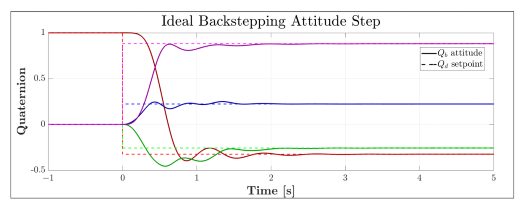
\includegraphics[width=0.65\textwidth]{graphs/IBC_Step}
\caption{Quaternion attitude step}
\label{fig:IBC_Step}
\end{subfigure}
\begin{subfigure}{0.49\textwidth}
\centering
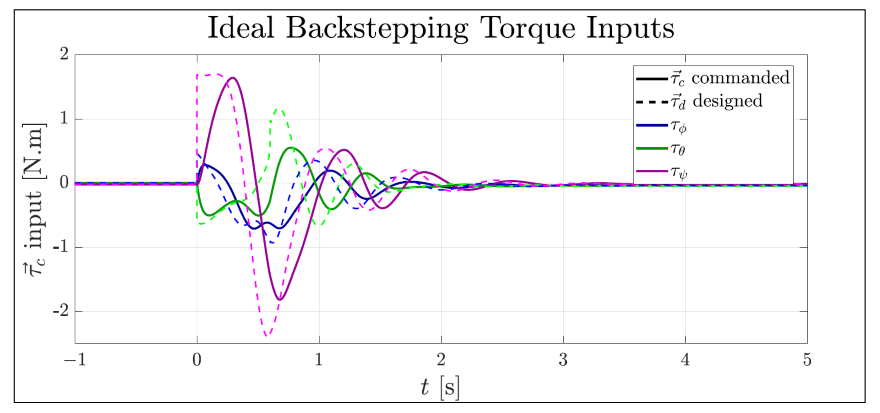
\includegraphics[width=\textwidth]{graphs/IBC_Torque}
\caption{Plant input torques}
\label{fig:IBC_Torque}
\end{subfigure}
\begin{subfigure}{0.49\textwidth}
\centering
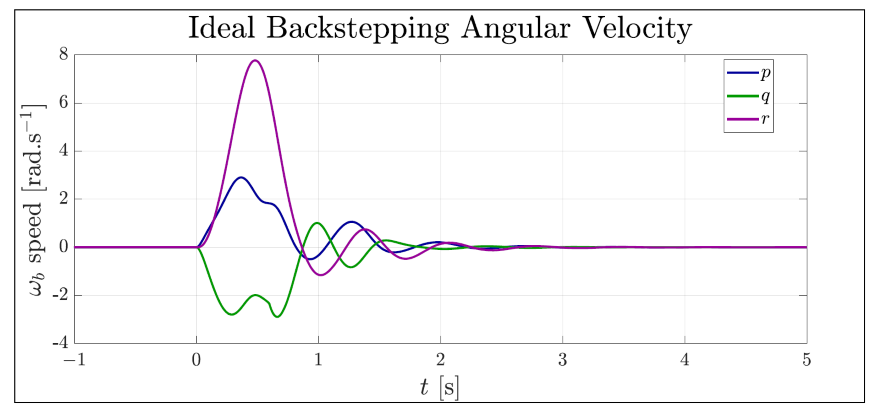
\includegraphics[width=\textwidth]{graphs/IBC_Angular}
\caption{Angular velocity}
\label{fig:IBC_Angular}
\end{subfigure}
\caption{Independent diagonal PD}
\end{figure}
\par
Adaptive backstepping is tested and discussed later in Sec:\ref{sec:simulation.disturbance.torque} in the context of robust stability, rather than controller performance\ldots 
%====================================================
\section{Position Controllers}
\label{sec:simulation.position}
%====================================================
Following the attitude controller optimization, a similar treatment was applied to the two proposed position control laws (Sec:\ref{sec:control.position}). It is important to specify that for position controller optimization a plant dependent diagonal PD attitude controller (Sec:\ref{subsubsec:simulation.atttiude.pd.dependent} was used to stabilize the coupled attitude dynamics. To test each position control coefficient swarm's performance the attitude setpoint was kept at a constant $Q_d=[1~\vec{0}]^T$, while various position setpoints were stepped. Moreover the same pseudo inversion allocator, Sec:\ref{subsec:allocation.allocators.inverse}, was used to test position control. Each position setpoint is defined in the inertial frame:
\begin{equation}
\vec{\mathcal{E}}_d(t)\triangleq\begin{bmatrix}
X_d(t)&
Y_d(t)&
Z_d(t)
\end{bmatrix}^T
~~~~\in\mathcal{F}^{I}
\end{equation}
A series of position setpoints were tested where each setpoint was positioned on the surface of a sphere at a radius of $C=5~[\text{m}]$ away from a central point. The starting position was consistently tested at $\vec{\mathcal{E}}_0=[5~5~5]^{T}~[\text{m}]$ relative to the origin. Each setpoint was distanced away from $\vec{\mathcal{E}}_0$:
\begin{equation}
\vec{\mathcal{E}}_d(t)=\vec{\mathcal{E}}_0+R_y(\theta_{y})R_x(\phi_{x})\begin{bmatrix}
0 & 0 & 5
\end{bmatrix}^T
\end{equation}
Where angles $\phi_x$ and $\theta_y$ rotate a radial arm for a range $\phi_x\in[-180\text{\textdegree}:180\text{\textdegree}]$ and $\theta_y\in[-90\text{\textdegree}:90\text{\textdegree}]$, both at intervals of $30~\text{\textdegree}$. That creates a position workspace sphere illustrated in Fig:\ref{fig:position-setpoint} with a possible 91 position setpoint to test.
\begin{figure}[htbp]
\centering
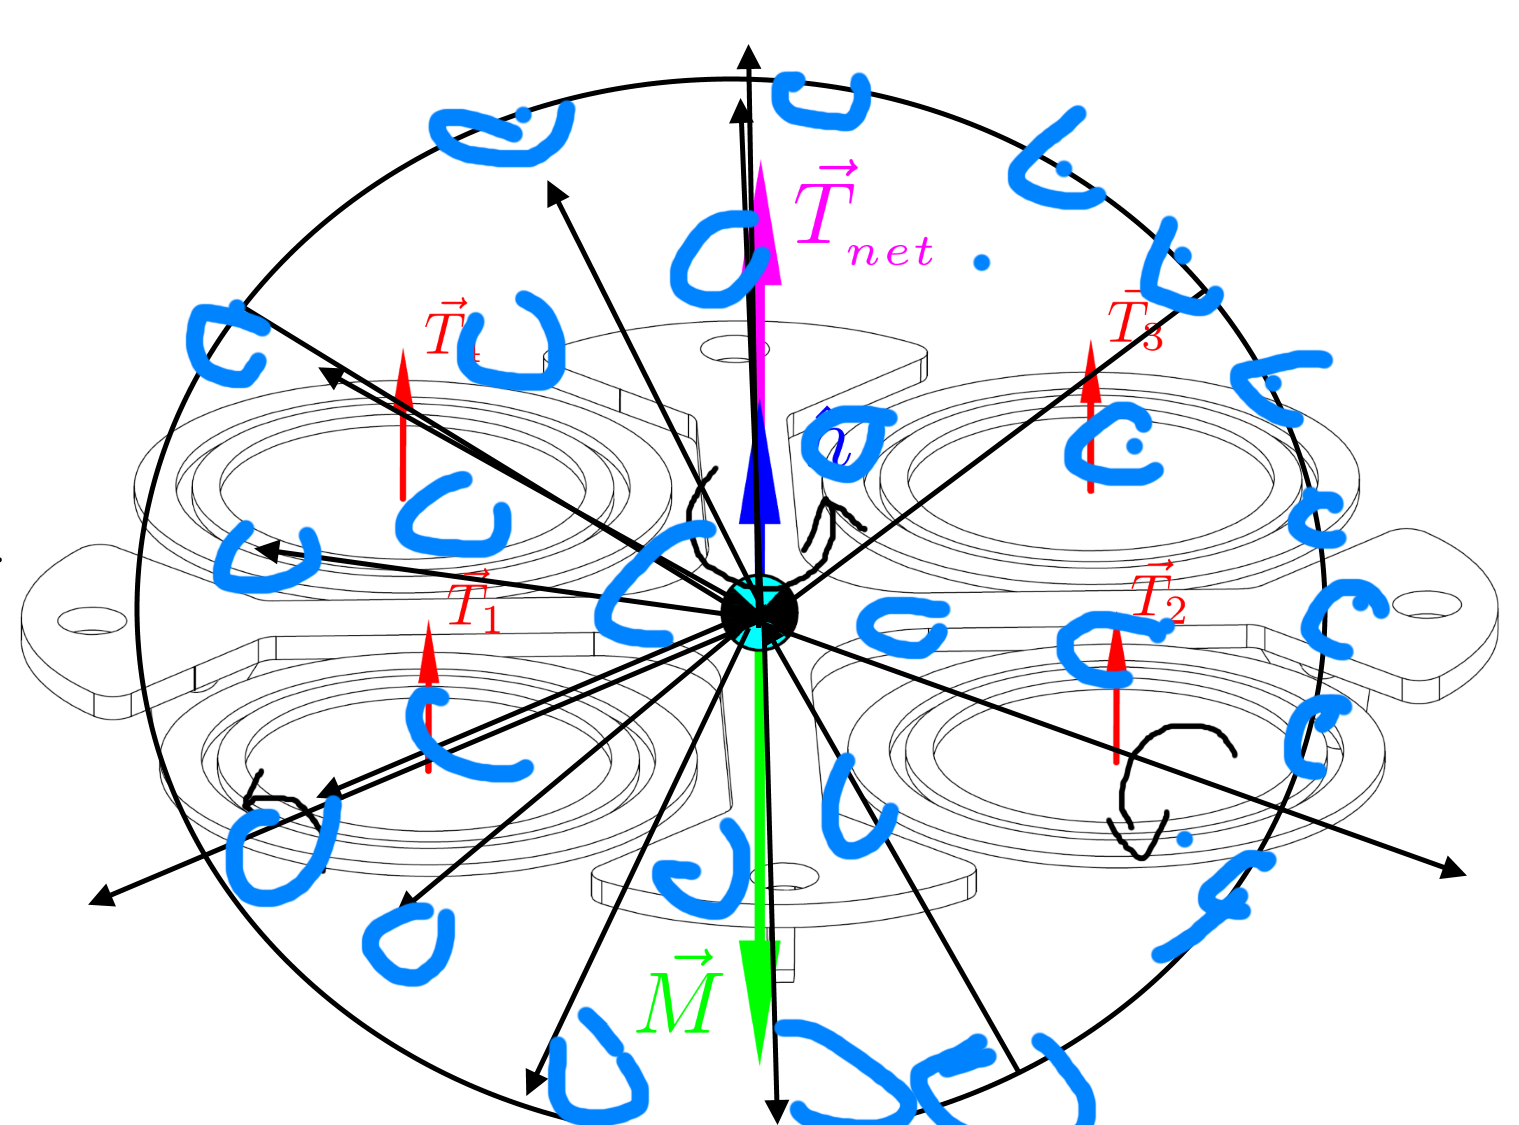
\includegraphics[width=0.7\textwidth]{figs/position-setpoint}
\caption{Position setpoint workspace}
\label{fig:position-setpoint}
\end{figure}
\par
Performance of each position step was another ITAE integral of the position error and translational velocity error, both transformed into the \emph{body frame}, $\mathcal{F}^{b}$. Again the simulation was given $t=15~[\text{s}]$ to reach it's settling point when stepped from the starting point.
\begin{equation}\label{eq:position-performance}
\vec{\zeta}_{\mathcal{E}}=C_{X}\int_{t=0}^{15}t|\vec{X}_e(t)|.dt+C_{v}\int_{t=0}^{15}t|\vec{v}_e(t)|.dt
\end{equation}
Weighting coefficients $C_X$ and $C_v$ priorities position and velocity errors respectively, but were both weighted equally such that $C_X=C_v=1$. Each swarm was tested 91 times and the resultant cost of Eq:\ref{eq:position-performance} was averaged for an overall performance metric. Only plant dependent compensating controllers were optimized for the position control loop. To compare the relative performance of position controllers a constant step test was applied in both cases:
\begin{equation}
\vec{\mathcal{E}}_d=\begin{bmatrix}
X_d\\
Y_d\\
Z_d
\end{bmatrix}=\begin{bmatrix}
7.5\\
4\\
3
\end{bmatrix}~~[\text{m}],~\in\mathcal{F}^{I}
\end{equation}
%====================================================
\subsection{PD}
\label{subsec:simulation.position.pd}
%====================================================
The reference case for position control is the Proportional-Derivative controller presented in Sec:\ref{subsec:control.position.pd}. Recalling that control structure:
\begin{equation}
\vec{F}_{_{PD}}=K_p\vec{X}_e + K_d\dot{\vec{X}}_e + \vec{\omega}_b\times m_b\vec{v}_b-m_b\vec{G}_b
\end{equation}
Where both $K_p$ and $K_d$ are diagonal gain coefficient matrices. The introduction of symmetric coefficients did not prove to be positive in Sec:\ref{subsubsec:simulation.atttiude.pd.3x3} so it was not pursued in the context of position control. Those coefficients are structured as follows:
\begin{equation}\label{eq:simulation-attitde-pd-diagonal-coefficients}
K_p\triangleq \begin{bmatrix}
K_p(1) & 0 & 0\\
0 & K_p(2) & 0\\
0 & 0 & K_p(3)
\end{bmatrix}
~~\text{and}~~K_d\triangleq \begin{bmatrix}
K_d(1) & 0 & 0\\
0 & K_d(2) & 0\\
0 & 0 & K_d(3)
\end{bmatrix}
\end{equation}
Each coefficient matrix acts on the position error, $\vec{X}_e$, and the velcoity error, $\vec{v}_e$ independently. As a result the local and global coefficient selections are simply:
\begin{equation}
\vec{P}_{Best}\equiv
\begin{bmatrix}
K_p(1)\Rightarrow \min \vec{X}_e(1)\\
K_p(2)\Rightarrow \min \vec{X}_e(2)\\
K_p(3)\Rightarrow \min \vec{X}_e(3)\\
K_d(1)\Rightarrow \min \vec{v}_e(1)\\
K_d(2)\Rightarrow \min \vec{v}_e(2)\\
K_d(3)\Rightarrow \min \vec{v}_e(3)
\end{bmatrix}~~\text{and}~~\vec{G}_{Best}\equiv\begin{bmatrix}
K_p(1)\Rightarrow \min \vec{\zeta}_{_{PD}}(1)\\
K_p(2)\Rightarrow \min \vec{\zeta}_{_{PD}}(2)\\
K_p(3)\Rightarrow \min \vec{\zeta}_{_{PD}}(3)\\
K_d(1)\Rightarrow \min \vec{\zeta}_{_{PD}}(1)\\
K_d(2)\Rightarrow \min \vec{\zeta}_{_{PD}}(2)\\
K_d(3)\Rightarrow \min \vec{\zeta}_{_{PD}}(3)
\end{bmatrix}
\end{equation}
The following optimized coefficients were produced:
\begin{equation}\label{eq:optimized-position-pd}
K_p = \begin{bmatrix}
2.4167 & 0 & 0\\
0 & 2.1557 & 0\\
0 & 0 & 2.5904
\end{bmatrix}
~~\text{and}~~K_d = \begin{bmatrix}
3.4794 & 0 & 0\\
0 & 3.3846 & 0\\
0 & 0 & 3.8698
\end{bmatrix}
\end{equation}
The inertial position step has a response shown in Fig:\ref{fig:PD_Position_Step}, stepping from the initial position to the setpoint described in Eq:\ref{eq:attitude-step-position}. The position settles in $t_{95}=4.6824~[\text{s}]$ without any overshoot. Not shown but still considered is the effect a step has on the attitude plant, which still remained stable at the origin. Because the attitude setpoint is $Q_d=[1~\vec{0}]^T$, most of the force requirement in Fig:\ref{fig:PD_Position_Force} is to oppose the gravitational downward force acting on the body.
\begin{figure}[htbp]
\centering
\begin{subfigure}{\textwidth}
\centering
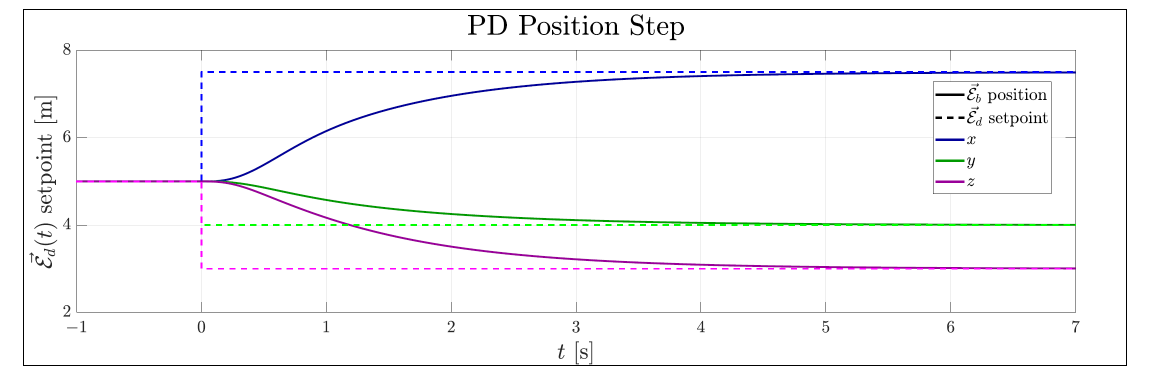
\includegraphics[width=0.65\textwidth]{graphs/PD_Position_Step}
\caption{Position step}
\label{fig:PD_Position_Step}
\end{subfigure}
\begin{subfigure}{0.49\textwidth}
\centering
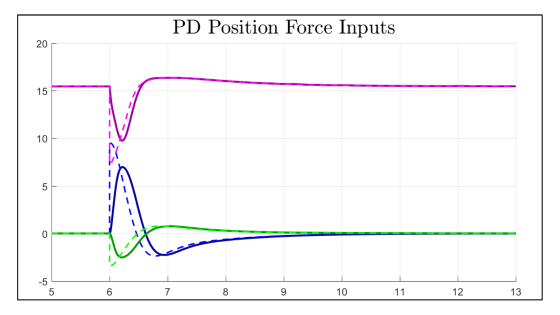
\includegraphics[width=\textwidth]{graphs/PD_Position_Force}
\caption{Plant input forces}
\label{fig:PD_Position_Force}
\end{subfigure}
\begin{subfigure}{0.49\textwidth}
\centering
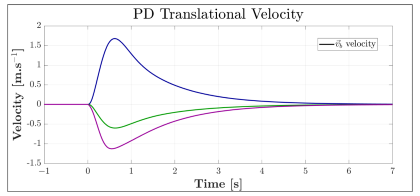
\includegraphics[width=\textwidth]{graphs/PD_Position_Velocity}
\caption{Position translational velocity}
\label{fig:PD_Position_Velocity}
\end{subfigure}
\caption{Position PD}
\end{figure}
\newpage
%====================================================
\subsection{Ideal and Adaptive Position Backstepping}
\label{subsec:simulation.position.pd}
%====================================================
The second, and final, position controller to be tested is that of the Ideal Backstabbing controller. Again the same coefficients are used for both the Ideal and Adaptive cases, the latter being evaluated subsequently in Sec:\ref{subsec:simulation.disturbance.force}. Recalling the position IBC structure from Sec:\ref{subsec:control.position.bacstepping}:
\begin{equation}\label{eq:simulation-position-IBC}
\vec{F}_{_{IBC}}=m_b\Big(\big(1+\Gamma_1\Gamma_2\big)\hat{z}_1-\big(\Gamma_1+\Gamma_2\big)\vec{v}_b\big)\Big)+\vec{\omega}_b\times m_b\vec{v}_b-m_b\vec{G}_b-\vec{D}_b
\end{equation}
The two coefficient gain matrices in Eq:\ref{eq:simulation-position-IBC} are both positive symmetric matrices. The coefficient structures are:
\begin{equation}\label{eq:simulation-position-diagonal-coefficients}
\Gamma_1\triangleq \begin{bmatrix}
\Gamma_1(1) & \Gamma_1(4) & \Gamma_1(5)\\
\Gamma_1(4) & \Gamma_1(2) & \Gamma_1(6)\\
\Gamma_1(5) & \Gamma_1(6) & \Gamma_1(3)
\end{bmatrix}
~~\text{and}~~\Gamma_2\triangleq \begin{bmatrix}
\Gamma_2(1) & \Gamma_2(4) & \Gamma_2(5)\\
\Gamma_2(4) & \Gamma_2(2) & \Gamma_2(6)\\
\Gamma_2(5) & \Gamma_2(6) & \Gamma_2(3)
\end{bmatrix}
\end{equation}
Both attitude and position ideal backstepping controllers have coefficients which act on both plant's error and error rates. This makes local and global coefficient position selection difficult without affecting the swarms optimization trajectory adversly. Again using $\Gamma_1$ to focus on optimizing position errors $\vec{X}_e$ and $\Gamma_2$ to settle velocity errors $\vec{v}_e$, the local and global best positions are chosen as follows:
\begin{subequations}
\begin{equation}
\vec{P}_{Best}\equiv
\begin{bmatrix}
\Gamma_1(1)\Rightarrow \min \vec{\mathcal{X}}_e(1) & \Gamma_1(4)\Rightarrow \min \vec{\mathcal{X}}_e(1)\&\&\vec{\mathcal{X}}_e(2)\\
\Gamma_1(2)\Rightarrow \min \vec{\mathcal{X}}_e(2)& \Gamma_1(5)\Rightarrow \min\vec{\mathcal{X}}_e(1)\&\&\vec{\mathcal{X}}_e(3) \\
\Gamma_1(3)\Rightarrow \min \vec{\mathcal{X}}_e(3) & \Gamma_1(6)\Rightarrow \min\vec{\mathcal{X}}_e(2)\&\&\vec{\mathcal{X}}_e(3)\\
\Gamma_2(1)\Rightarrow \min \vec{v}_e(1) & \Gamma_2(4)\Rightarrow \min\vec{v}_e(1)\&\&\vec{v}_e(2)\\
\Gamma_2(2)\Rightarrow \min \vec{v}_e(2) & \Gamma_2(5)\Rightarrow\min\vec{v}_e(1)\&\&\vec{v}_e(3)\\
\Gamma_2(3)\Rightarrow \min \vec{v}_e(3)& \Gamma_2(6)\Rightarrow\min\vec{v}_e(2)\&\&\vec{v}_e(3)
\end{bmatrix}
\end{equation}
\begin{equation}
\vec{G}_{Best}\equiv\begin{bmatrix}
\Gamma_1(1)\Rightarrow \min \vec{\zeta}_{_{IBC}}(1) & \Gamma_1(4)\Rightarrow\min\vec{\zeta}_{_{IBC}}(1)\&\& \vec{\zeta}_{_{IBC}}(2)\\
\Gamma_1(2)\Rightarrow \min \vec{\zeta}_{_{IBC}}(2) & \Gamma_1(5)\Rightarrow\min\vec{\zeta}_{_{IBC}}(1)\&\& \vec{\zeta}_{_{IBC}}(3)\\
\Gamma_1(3)\Rightarrow \min \vec{\zeta}_{_{IBC}}(3) & \Gamma_1(6)\Rightarrow\min\vec{\zeta}_{_{IBC}}(2)\&\& \vec{\zeta}_{_{IBC}}(3)\\
\Gamma_2(1)\Rightarrow \min \vec{\zeta}_{_{IBC}}(1) & \Gamma_2(4)\Rightarrow\min\vec{\zeta}_{_{IBC}}(1)\&\& \vec{\zeta}_{_{IBC}}(2)\\
\Gamma_2(2)\Rightarrow \min \vec{\zeta}_{_{IBC}}(2) & \Gamma_2(5)\Rightarrow\min\vec{\zeta}_{_{IBC}}(1)\&\& \vec{\zeta}_{_{IBC}}(3)\\
\Gamma_2(3)\Rightarrow \min \vec{\zeta}_{_{IBC}}(3) & \Gamma_2(6)\Rightarrow\min\vec{\zeta}_{_{IBC}}(2)\&\& \vec{\zeta}_{_{IBC}}(3)\\
\end{bmatrix}
\end{equation}
\end{subequations}
The optimized gain coefficients for $\Gamma_1$ and $\Gamma_2$ were then produced by the PSO algorithm:
\begin{equation}\label{eq:optimized-Position-IBC}
\Gamma_1 = \begin{bmatrix}
2.3409 & 0.17071 & -0.16444\\
0.17071 & 2.0493 & 0.10597\\
-0.16444 & 0.10597 & 1.7322
\end{bmatrix}
~~\text{and}~~\Gamma_2= \begin{bmatrix}
1.5287 & 0.029275 & 0.081552\\
0.029275 & 1.4214 & -0.041008\\
0.081552 & -0.041008 & 1.4753
\end{bmatrix}
\end{equation}
\par
\begin{figure}[hbtp]
\vspace{-15pt}
\centering
\begin{subfigure}{\textwidth}
\centering
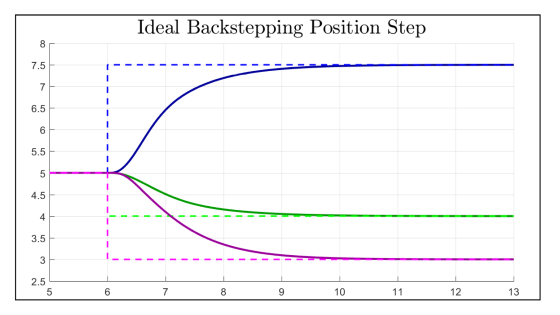
\includegraphics[width=0.65\textwidth]{graphs/IBC_Position_Step}
\caption{Position step}
\label{fig:IBC_Position_Step}
\end{subfigure}
\end{figure}
\newpage
\begin{figure}[htbp]\ContinuedFloat
\begin{subfigure}{0.49\textwidth}
\centering
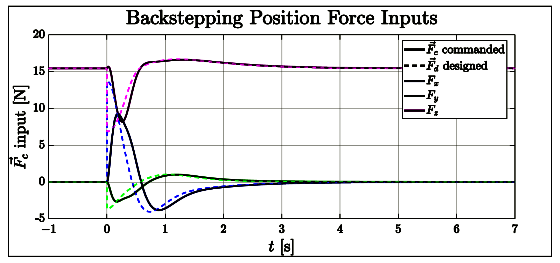
\includegraphics[width=\textwidth]{graphs/IBC_Position_Force}
\caption{Plant input forces}
\label{fig:IBC_Position_Force}
\end{subfigure}
\begin{subfigure}{0.49\textwidth}
\centering
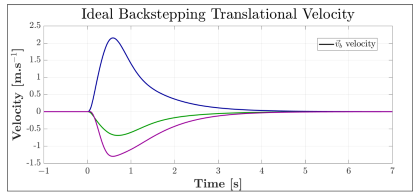
\includegraphics[width=\textwidth]{graphs/IBC_Position_Velocity}
\caption{Position translational velocity}
\label{fig:IBC_Position_Velocity}
\end{subfigure}
\caption{Position Backstepping Controller}
\end{figure}
\par
Fig:\ref{fig:IBC_Position_Step} shows the step response to a change in translational position setpoint. Note that the position plotted in Fig:\ref{fig:IBC_Position_Step} is the relative position in the inertial frame $\mathcal{F}^{I}$. The Ideal Backstepping controller settles in $t_{95}=3.1057~[\text{s}]$, showing the improvement exponential stability applies to the asymptotic stability achieved by a PD controller previously\ldots
\par
It is not unexpected that with faster settling times greater input control requirements, the virtual and commanded input forces in Fig:\ref{fig:IBC_Position_Force} are far greater than those previously in Fig:\ref{fig:PD_Position_Force}. For the most part the velocity step in Fig:\ref{fig:IBC_Position_Velocity} follows a smooth rate change.
%====================================================
\section{Set-point Control Results}
\label{sec:simulation.autopilot}
%====================================================
Each of the controllers were respectively stable in their own right. The trajectory used to corroborate dynamic setpoint tracking, illustrated in Fig:\ref{fig:trajectory}, is not a complex one. A slow orbital velocity of $\dot{\theta}=0.5~[\text{Hz}]$ was applied, completing one orbit around the central $\vec{C}_0$ every $120~[\text{s}]$. What follows is each attitude's and position controllers performance tracking that particular trajectory. 
\par
Only the plant dependent, diagonal Proporitional derivative attitude controller was tested here. Sec:\ref{subsec:simulation.attitude.pd} showed that plant dependency was a necessity and that a symmetric coefficient controller provided no improvement. Adaptive backstepping controllers and their disturbance rejection properties are discussed next in Sec:\ref{sec:simulation.disturbnace}.
\par
Each attitude controller was tested together with a shared PD position controller, tracking the orbital XYZ position. Conversely each position controller is tested using a simple diagonal PD controller to track the attitude. The attitude controllers have an initial step to reach the orbital attitude from a starting point $Q_0=[1~\vec{0}]^T$. Each control law was successful in tracking a given trajectory, not much insight can be gained from an in-depth discussion as the results are decidedly similar\ldots
\begin{figure}[hbtp]
\begin{subfigure}{\textwidth}
\centering
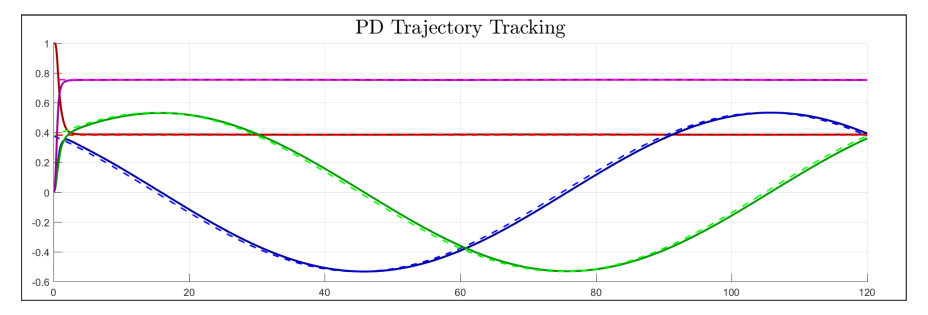
\includegraphics[width=0.85\textwidth]{graphs/PD_Diagonal_Dependent_Trajectory}
\caption{Diagonal Proportional Derivative Controller}
\end{subfigure}
\end{figure}
\par
\begin{figure}[hbtp]\ContinuedFloat
\vspace{-6pt}
\begin{subfigure}{\textwidth}
\centering
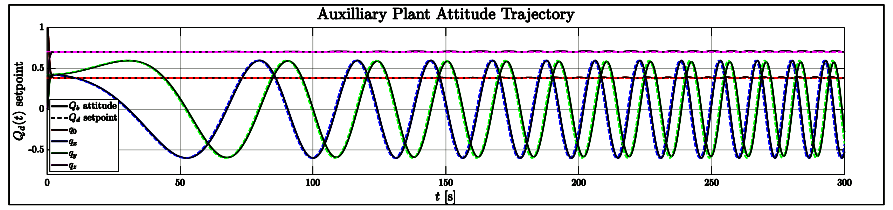
\includegraphics[width=0.85\textwidth]{graphs/XPD_Trajectory}
\vspace{-6pt}
\caption{Auxiliary Plant Controller}
\end{subfigure}
\vspace{-6pt}
\begin{subfigure}{\textwidth}
\centering
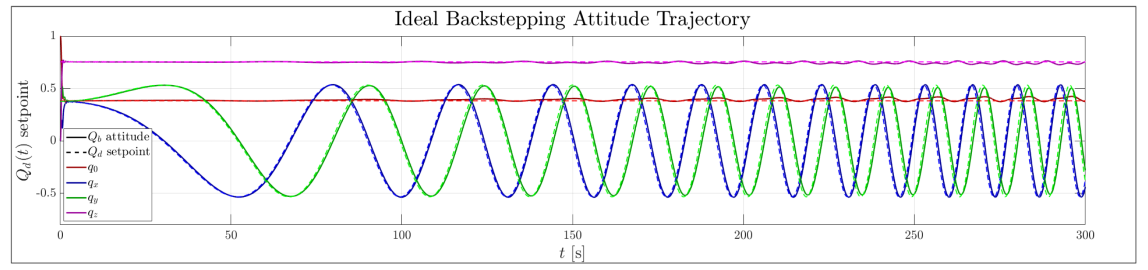
\includegraphics[width=0.85\textwidth]{graphs/IBC_Trajectory}
\vspace{-6pt}
\caption{Ideal Backstepping Controller}
\label{fig:attitude-trajectory-ibc-tracking}
\end{subfigure}
\caption{Attitude Trajectory Tracking}
\label{fig:attitude-trajectory-tracking}
\vspace{-20pt}
\end{figure}
\par
\hspace{2pt}\vspace{20pt}
\par
\begin{figure}[hbtp]
\vspace{-40pt}
\begin{subfigure}{\textwidth}
\centering
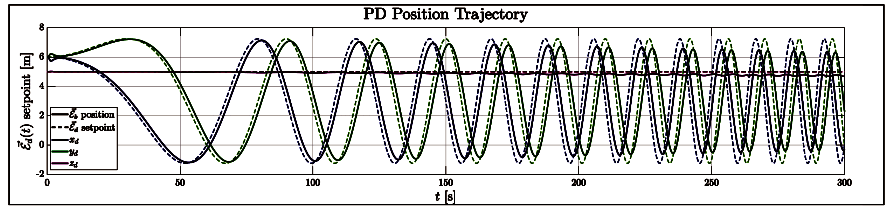
\includegraphics[width=0.85\textwidth]{graphs/PD_Position_Trajectory}
\vspace{-6pt}
\caption{Diagonal Proportional Derivative Controller}
\end{subfigure}
\vspace{-6pt}
\begin{subfigure}{\textwidth}
\centering
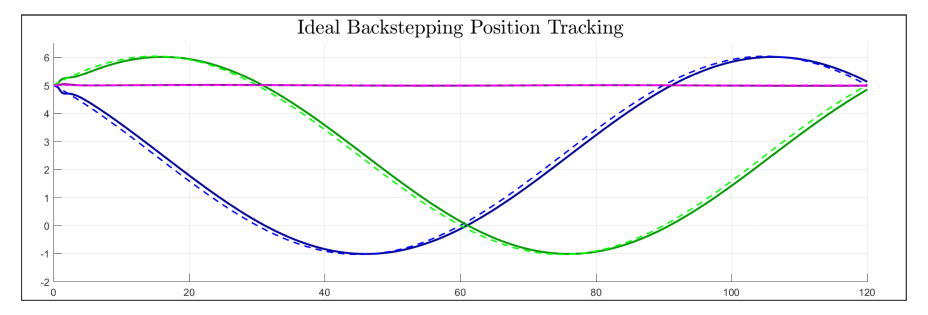
\includegraphics[width=0.85\textwidth]{graphs/IBC_Position_Trajectory}
\vspace{-6pt}
\caption{Ideal Backstepping Controller}
\end{subfigure}
\caption{Position Trajectory Tracking}
\label{fig:position-trajectory-tracking}
\vspace{-24pt}
\end{figure}
\par
\vspace{14pt}
The only difference between attitude controllers in Fig:\ref{fig:attitude-trajectory-tracking} is that the ideal backstepping attitude controller, Fig:\ref{fig:attitude-trajectory-ibc-tracking}, has an oscillatory response to the initial step in attitude. There is a slight phase lag, most prominent in the position controllers in Fig:\ref{fig:position-trajectory-tracking}, this is as a result of only first order setpoint tracking. If velocities were generated together with a trajectory setpoint then that phase delay would be diminished\ldots
\newpage
%====================================================
\section{Robust Stability and Disturbance Rejection}
\label{sec:simulation.disturbnace}
%====================================================
Despite deriving adaptive control laws in Sec:\ref{subsubsec:control.attitude.nonlinear.adaptivebackstep} and Sec:\ref{subsec:control.position.bacstepping} for attitude and position controllers; each of the proposed controller laws demonstrated acceptable stability under sizeable disturbances. App:\ref{app:disturbance} shows each controller's trajectory response to uncompensated disturbances acting on the vehicle. The torque and force disturbances are described subsequently\ldots
%====================================================
\subsection{Torque Disturbance Rejection}
\label{subsec:simulation.disturbance.torque}
%====================================================
Typical turbulence torques are difficult to define without in-depth statistical and mathematical analysis. To expedite the stability/disturbance evaluation process, torque turbulences were approximated using a Dryden Gust model,\cite{optimalgust,discretegustmodel}. Alternatively the Von Karman aerospace disturbance model(s) could be implemented but are computationally more exhaustive.
\par
Without going into too much detail, the Dryden Wind model produces spectral turbulences from white noise filtered through a specified Dryden power spectrum. That power spectrum varies as per an aircraft's orientation, altitude and translational velocity. In general, for the aircraft and trajectory under consideration here, such a disturbance model is sufficient for producing small interference patterns\ldots
\begin{equation}\label{eq:stability-torque-overserver}
\dot{\hat{L}}=-\Gamma_L J_b^{-1}(u)\big(\Gamma_1\vec{q}_e-\vec{\omega_b}\big)
\end{equation}
The gain adaptivity matrix $\Gamma_L$ was optimized on steady state such that the observer's error was minimized; resulting in a value of $\Gamma_L=diag(29.58,~28.43,~4.60)$. Eq:\ref{eq:stability-torque-overserver} recalls the torque disturbance observer model from Eq:\ref{eq:asymptotic-disturbance}, Fig:\ref{fig:torque-observer} plots how the approximator tracks torque disturbances in the range of $\pm 0.2~[\text{N.m}]$ over a short steady state test. 
\begin{figure}[htbp]
\vspace{-6pt}
\centering
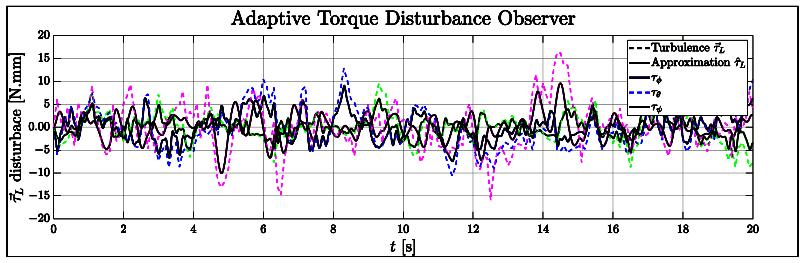
\includegraphics[width=0.8\textwidth]{graphs/torque-observer}
\caption{Attitude torque disturbance observer}
\vspace{-18pt}
\label{fig:torque-observer}
\end{figure}
\par
Fig:\ref{fig:ABC_trajectory} then plots the adaptive backstepping controller attitude over an entire orbital trajectory. A slight improvement over an uncompensated IBC controller, shown in Fig:\ref{fig:app-attitude-ibc-dist} from App:\ref{app:disturbance}. The cost of the disturbance approximator in the attitude plant is faster fluctuating input torques which could indeed reach actuator rate saturation.
\begin{figure}[hbtp]
\vspace{-6pt}
\centering
\includegraphics[width=0.8\textwidth]{graphs/ABC_trajectory}
\caption{Adaptive backstepping attitude trajectory tracking}
\label{fig:ABC_trajectory}
\vspace{-16pt}
\end{figure}
%====================================================
\subsection{Disturbance Force Rejection}
\label{subsec:simulation.disturbance.force}
%====================================================
Force disturbance is similarly simulated using a Dryden Gust model for wind turbulent velocity generation. A wind vector field across the inertial frame test space was also introduced to add an effective constant force offset throughout the vehicles trajectory simulation. Recalling the force disturbance observer from Eq:\ref{eq:abc-asymptotic-position}, each estimate is updated such that:
\begin{equation}
\dot{\hat{D}}=-m_b^{-1}\Gamma_D\Big(\Gamma_1\hat{z}_1-\vec{v}_b\Big)
\end{equation}
Where $\Gamma_D$ is the force disturbance observer's adaptivity gain matrix. Using $\Gamma_D=diag(4.203,~3.840,~3.971)$ the observer tracks a force disturbance acting on the vehicle over a range of $-4\rightarrow 8~[N]$. Fig:\ref{fig:force-observer} shows the force observer adapting over an entire simulation to illustrate the vector field effects\ldots
\begin{figure}[hbtp]
\vspace{-6pt}
\centering
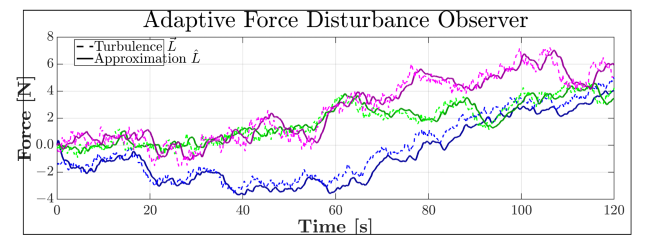
\includegraphics[width=0.8\textwidth]{graphs/force-observer}
\caption{Position force disturbance observer}
\label{fig:force-observer}
\vspace{-16pt}
\end{figure}
\par
The position adaptive backstepping controller then tracks the inertial frame trajectory as shown in Fig:\ref{fig:ABC_Position_Trajectory}. Again improving the trajectory tracking performance slightly when compared to the Ideal backstepping case from Fig:\ref{fig:app-position-ibc-dist}; but even without adaptive disturbance compensation, the plant is stable throughout the trajectory albeit somewhat noisy\ldots
\begin{figure}[hbtp]
\centering
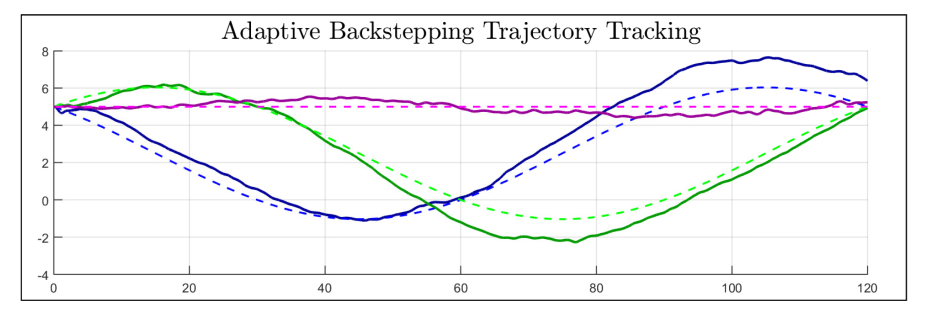
\includegraphics[width=0.8\textwidth]{graphs/ABC_Position_Trajectory}
\caption{Adaptive backstepping position trajectory tracking}
\label{fig:ABC_Position_Trajectory}
\end{figure}
%====================================================
\section{Allocation Tests}
\label{sec:simulation.allocator}
%====================================================

%====================================================
\section{Input Saturation}
\label{sec:simulation.saturation}
%====================================================

%====================================================
\section{State Estimation}
\label{sec:simulation.state}
%====================================================

